\documentclass[
  captions=tableheading,
  bibliography=totoc, 
  titepage=firstiscover,
]{scrartcl}

\usepackage{blindtext} %neuer input

\usepackage{longtable} % Tabellen über mehrere Seiten

\usepackage[utf8]{inputenc} %neuer input

\usepackage{scrhack}

\usepackage[aux]{rerunfilecheck} %Warnung falls nochmal kompiliert werden muss

\usepackage{fontspec} %Fonteinstellungen

\recalctypearea{}

\usepackage[main=ngerman]{babel} %deutsche Spracheinstellung

\usepackage{ragged2e} %neuer input

\usepackage{amsmath, nccmath}

\usepackage{amssymb} %viele mathe Symbole

\usepackage{mathtools} %Erweiterungen für amsmath


\DeclarePairedDelimiter{\abs}{\lvert}{\rvert}
\DeclarePairedDelimiter{\norm}{\lVert}{\rVert}

\DeclarePairedDelimiter{\bra}{\langle}{\rvert}
\DeclarePairedDelimiter{\ket}{\lvert}{\rangle}

\DeclarePairedDelimiterX{\braket}[2]{\langle}{\rangle}{
#1 \delimsize| #2
}

\NewDocumentCommand \dif {m}
{
\mathinner{\symup{d} #1}
}


\usepackage[
  math-style=ISO,
  bold-style=ISO,
  sans-style=italic,
  nabla=upright,
  partial=upright,
  warnings-off={
    mathtools-colon,
    mathtools-overbracket,
  },
]{unicode-math}

\setmathfont{Latin Modern Math}
\setmathfont{XITS Math}[range={scr, bfscr}]
\setmathfont{XITS Math}[range={cal, bfcal}, StylisticSet=1]


\usepackage[
  locale=DE,
  separate-uncertainty=true,
  per-mode=reciprocal,
  output-decimal-marker={,},
]{siunitx}

\usepackage[autostyle]{csquotes} %richtige Anführungszeichen

\usepackage{xfrac}

\usepackage{float}

\floatplacement{figure}{htbp}

\floatplacement{table}{htbp}

\usepackage[ %floats innerhalb einer section halten
  section,   %floats innerhalb er section halten
  below,     %unterhalb der Section aber auf der selben Seite ist ok
]{placeins}

\usepackage[
  labelfont=bf,
  font=small,
  width=0.9\textwidth,
]{caption}

\usepackage{subcaption} %subfigure, subtable, subref

\usepackage{graphicx}

\usepackage{grffile}

\usepackage{booktabs}

\usepackage{microtype} %Verbesserungen am Schriftbild

\usepackage[
backend=biber,
]{biblatex}

\addbibresource{../lit.bib}

\usepackage[ %Hyperlinks im Dokument
  german,
  unicode,
  pdfusetitle,
  pdfcreator={},
  pdfproducer={},
]{hyperref}

\usepackage{bookmark}

\usepackage[shortcuts]{extdash}

%\usepackage{warpcol}

\usepackage{tikz}

\newcommand*\circled[1]{\tikz[baseline=(char.base)]{
            \node[shape=circle,draw,inner sep=2pt] (char) {#1};}}

\begin{document}
    \title{V703: Das Geiger-Müller Zählrohr}
    \author{  
    Paul Störbrock\\
    \texorpdfstring{\href{mailto:paul.stoerbrock@tu-dortmund.de}{paul.stoerbrock@tu-dortmund.de}}{}
    }
    \date{Abgabe: 26.05.2020\vspace{-4ex}}
\maketitle
    
\newpage
\tableofcontents
\newpage

\setcounter{page}{1}

\section{Ziel}

    \flushleft{Das\;}\justifying Ziel dieses Versuches ist die Totzeit eines Geiger-Müller Zählrohrs zu bestimmen. Dazu werden die 
    Zählrohrcharakteristik und die Anzahl der freigesetzten Ladungen pro einfallendem Teilchen untersucht. 

\section{Theorie}

    \flushleft{Das\;}\justifying Geiger-Müller Zählrohr wird in der Physik verwendet, um
    ionisierende Strahlung zu Messen. Dabei werden durch die Absorption von $\alpha$- und
    $\beta$-Teilchen, und Röntgen-Quanten elektrische Impulse erzeugt, die mit dem 
    richtigen Aufbau gemessen werden können. Der Querschnitt eines Geiger-Müller Zählrohrs
    ist in der folgenden Abbildung dargestellt:

    \begin{figure}[H]
        \centering
        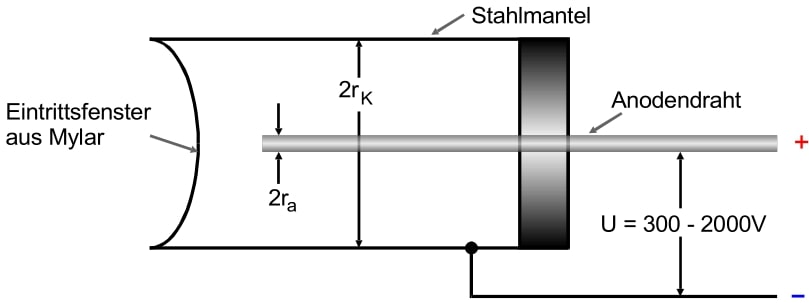
\includegraphics[width=\linewidth]{images/Querschnitt.jpg}
        \caption{Aufbau eines Geiger-Müller Zählrohrs \cite{V703}}
        \label{fig:1}
    \end{figure}

    \flushleft{Die\;}\justifying einfallenden Teilchen wandern durch das Eintrittsfenster
    in den Hohlraum des Zählrohrs. Der Hohlraum ist mit einem Gasgemisch (z.B.
    $\SI{100}{\milli\bar}$ Argon und $\SI{100}{\milli\bar}$ Ethylalkohol) gefüllt. 
    Wird zwischen Stahlmantel (Kathode) und dem Anodendraht eine Spannung aufgebaut, 
    entsteht im Hohlraum ein radialsymmetrisches Feld. Dieses Feld beschleunigt die
    eintretenden Teilchen in Richtung des Anodendrahts wie $\sfrac{1}{r}$, wobei bei
    einem bliebig kleinen Radius $r_a$ mit $r_a < r < r_k$ die Beschleunigung unendlich
    groß werden kann. 

    \flushleft{Das\;}\justifying hat zur Folge, dass ein einfallendes Teilchen das
    Gasgemisch solange ionisiert, bis dessen gesamte Energie aufgebraucht ist. Die
    nun freien Elektronen wandern zum Anodendraht, können jedoch auf dem Weg
    rekombiniert werden. Da die Zahl der gewonnenen Elektronen und Ionen proportional
    zur Energie des einfallenden Teilchens ist, ist auch der gemessene Ionisationsstrom
    proportional zur Intensität der Strahlung. Außerdem kann die Zahl der Rekombination 
    verringert werden, indem das E-Feld, also die angelegte Spannung erhöht wird. Demnach 
    ist der Ionisationsstrom auch proportional zur Feldstärke des E-Felds. Die Abhängigkeit 
    zwischen Spannung und Elektron-Ionen-Paare wird in der folgenden Abbildung verdeutlicht:

    \begin{figure}[H]
        \centering
        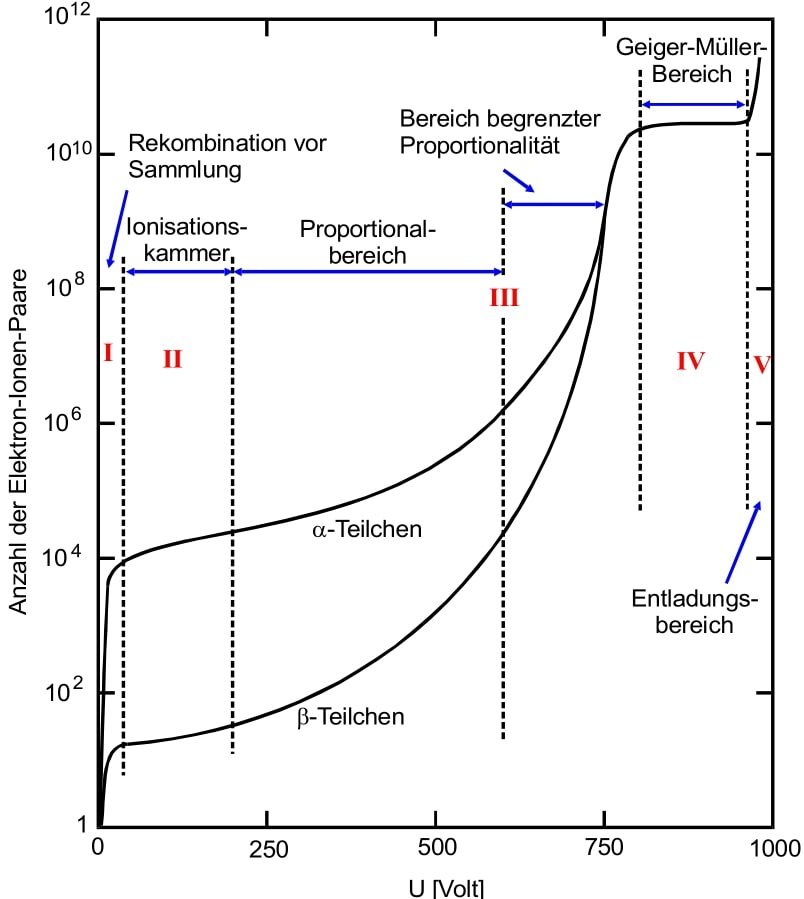
\includegraphics[width=0.75\linewidth]{images/Messbereich.jpg}
        \caption{Anzahl der Elektron-Ionenpaare als Funktion der Spannung $U$ \cite{V703}}
        \label{fig:2}
    \end{figure}

    \flushleft{Bei\;}\justifying außreichender Strahlung und relativ geringer Spannung wird
    der in Abbildung \ref{fig:1} gezeigte Aufbau als Ionisationskammer Bezeichnet (\ref{fig:2}
    Bereich II). Wird die Spannung jedoch weiter erhöht, gewinnen die Elektronen, die vom 
    einfallenden Teilchen aus den Argon-Atomen gelöst wurden, durch das E-Feld nahe des 
    Anodendrahts genug Energie, um selbst Atome zu ionisieren. Dieser Vorgang wird als 
    Stoßionisation bezeichnet und hat einen Lawinen-Effekt zur Folge (Townsend-Lawine), die
    genügend Ladung am Anodendraht sammelt um den elektrischen Ladungsimpuls messen zu können. Hierbei
    ist zu berücksichtigen, dass die Ladung immer noch proportional zur abgegebenen Energie des
    einfallenden Teilchens ist. Folglich kann der Ladungsimpuls als Maß der Teilchenenergie benutzt
    werden. Aus der Proportionalität folgt der Name des Bereichs III in Abbildung \ref{fig:2}.

    \flushleft{In\;}\justifying Abbildung \ref{fig:2} wird außerdem deutlich, dass der 
    Proportionalitätsbereich bei einer genügend hohen Spannung endet. Der Bereich IV ist hier
    der wichtige Bereich, da das Geiger-Müller Zählrohr in diesem Bereich arbeitet. Im Bereich
    IV ist die Spannung so groß und das E-Feld so stark, dass durch die Townsend-Lawine auch 
    UV-Photonen emittiert werden. Da Photonen neutral geladen sind, werden sie nicht vom E-Feld
    zum Anodendraht geschickt und können sich auch senkrecht zu den Feldlinien ausbreiten. Diese 
    Bewegungsfreiheit hat zur Folge, dass sich im gesamten Hohlraum Elektronenlawinen bilden. 
    Nun hängt die Ladung nicht mehr von der Energie des einfallenden Teilchens ab, weshalb der
    Ladungsimpuls nur noch als Maß der Intensität verwendet werden kann (Geiger-Müller Zählrohr).
    Durch die erhöhte Elektronenzahl in dem großen Ionisationsstrom wandern freie Elektronen 
    relativ schnell zum Anodendraht. Massereichere, positiv geladene Ionen hingegen verweilen
    länger im Hohlraum und bauen langsam einen \"Ionen-Schlauch\"\; auf, der die Feldstärke am 
    Anodendraht reduziert. Ist die Feldstärke klein genug, kann keine Stoßionisation mehr
    stattfinden, was bedeutet, dass ein neu einfallendes Teilchen nicht mehr registriert werden
    kann. Dieser Zeitpunkt $T$ wird als Totzeit bezeichnet und in der folgenden Abbildung dargestellt:

    \begin{figure}[H]
        \centering
        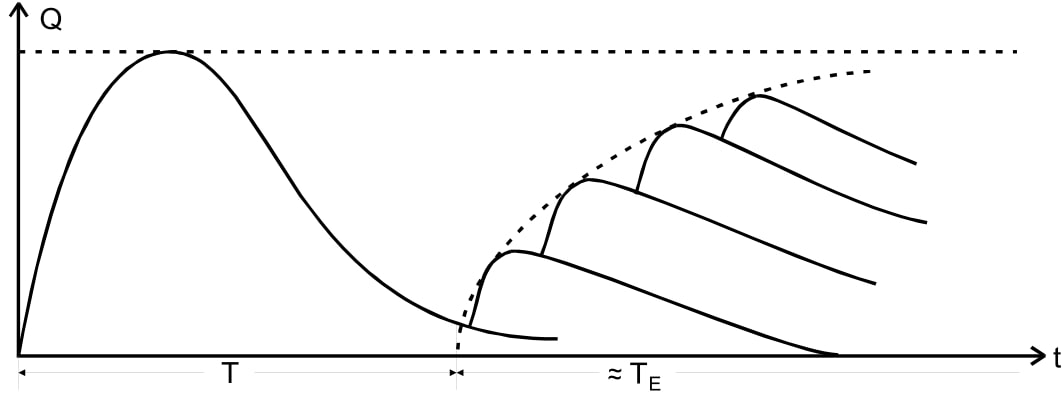
\includegraphics[width=\linewidth]{images/Erholungszeit.jpg}
        \caption{Tot- und Erholungszeit als Ladungs-Zeit-Diagramm \cite{V703}}
        \label{fig:3}
    \end{figure}

    \flushleft{Über\;}\justifying die Totzeit wandern die Ionen zum Stahlmantel und das E-Feld wird
    langesam wieder aufgebaut. Die Dauer dieses Prozesses $T_E$ heißt Erholungszeit und wird durch
    die Einhüllende der Energieschübe, die in Abbildung \ref{fig:3} abgebildet werden, dargestellt.
    Diese Energieschübe entstehen, da die Ionen beim Auftreffen auf den Stahlmantel neutralisiert 
    werden und genug Energie freisetzen um die Austrittsarbeit der Elektronen zu überwinden. Die
    aus dem Stahlmantel herausgelösten Elektron wandern zum Anodendraht und können auf dem Weg 
    neue und zeitlich versetzte Zählrohrentladungen auslösen. Diese zeitlich versetzten Ladungsstöße
    heißen Nachentladungen und sind in Abbildung \ref{fig:3} unter der Einhüllenden deutlich erkennbar.
    Die Nachentladung störrt und kann mit dem Zusatz von Ethylalkohol größtenteils behoben werden, da 
    Ethylalkoholionen während der Neutralisierung an dem Stahlmantel nicht genug Energie aufbringen 
    können, um Elektronen zu lösen. 

    \newpage
    \flushleft{Um\;}\justifying die Charakteristik eines Zählrohrs zu bestimmen, wird die Intensität
    $N$ gegen die angelegte Spannung $U$ aufgetragen. Der daraus folgende Graph

    \begin{figure}[H]
        \centering
        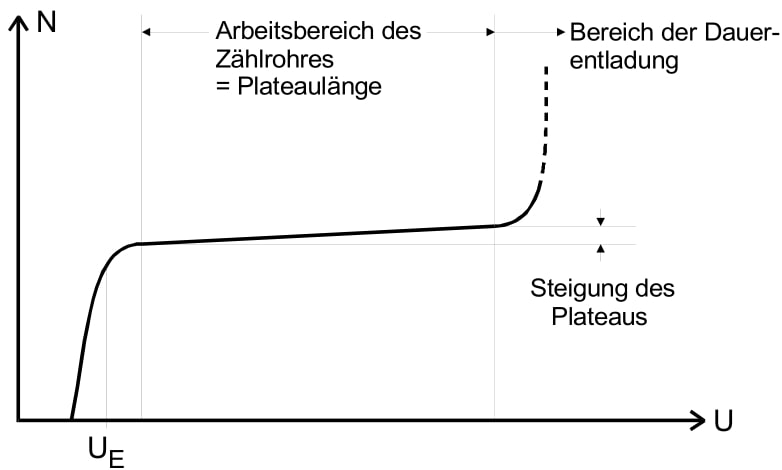
\includegraphics[width=\linewidth]{images/Plateau.jpg}
        \caption{Graphische Darstellung der Zählrohrcharakteristik \cite{V703}}
        \label{fig:4}
    \end{figure}

    \flushleft{stellt\;}\justifying das Plateau eines Zählrohrs dar. Das Plateau hat im idealen Fall
    eine Steigung von $0$, doch kann eine Nachentladung selbst durch das vorliegende Gasgemisch nicht
    vermieden werden. $U_E$ ist hier die Spannung, an welcher das Gasgemisch ionisiert wird. Die länger
    des Plateaus ist ein Qualitätsmaß des Zählrohrs. Hinter dem Plateau geht der Graph in den Bereich
    der Dauerentladung über. In diesem Bereich (Bereich V in Abbildung \ref{fig:2}) hat besitzt das 
    ionisierende Teilche genug Energie um eine Dauerentladung zu zünden. Die dabei entstehenden hohen 
    Stromdichten können das Zählrohr zerstören.

    \flushleft{Die\;}\justifying Totzeit $T$ wird hier über zwei Methoden bestimmt: die Zwei-Quellen-
    Methode (ZQM) und die Oszilloskopmethode (OM). Die ZQM vergleicht die Impulsraten zweier Quellen
    indem die Impulsraten $N$ beider Quellen jeweils einmal separat ($N_1, N_2$) und einmal zusammen 
    ($N_{1+2}$) gemessen werden. Dabei wird beachtet, dass auf Grund der Totzeit $T$ die gemessene 
    Impulsrate $N_r$ immer kleiner ist, als die tatsächliche Teilchenzahl $N_w$, die im Zählrohrvolumen 
    absorbiert werden.

    \newpage
    \flushleft{Aus\;}\justifying der tatsächlichen Teilchenzahl \cite{V703}
    \begin{align}
        N_w &= \frac{Impulsrate}{Messzeit} = \frac{N_r t}{(1-TN_r)t} = \frac{N_r}{1-TN_r} \label{eq:1}
    \end{align}
    \flushleft{folgt\;}\justifying für die drei Impulsraten $N_1,N_2,N_{1+2}$ unter der Bedingung
    $N_{1+2} = N_1+N_2$ die Gleichung:
    \begin{align}
        \frac{N_{1+2}}{1-TN_{1+2}} &= \frac{N_1}{1-TN_1}+\frac{N_2}{1-TN_2} \label{eq:2}
    \end{align}
    \flushleft{Diese\;}\justifying Gleichung kann nach $T$ umgestellt werden, wodurch die Totzeit als
    \begin{align}
        T &\approx \frac{N_1+N_2-N_{1+2}}{2N_1N_2} \label{eq:3}
    \end{align}
    \flushleft{approximiert\;}\justifying werden kann. Die Totzeit kann nicht definitiv bestimmt werden,
    da die Bedingung $N_{1+2} = N_1+N_2$ durch trotzdem auftretenden Nachentladungen experimentell zu $N_{1+2} < N_1+N_2$ korrigiert wird. 

    \flushleft{Die\;}\justifying Zahl der freigesetzten Ladungen pro einfallendem Teilchen $Z$ kann mit den 
    Zählrohrstrom $I$ wie folgt berechnet werden: \cite{V703}
    \begin{align}
        Z &= \frac{I}{e_0 N} \label{eq:5}
    \end{align}
    \flushleft{Wobei\;}\justifying $e_0$ die Elementarladung eines Elektrons und $N$ die Impulszahl darstellt.

\newpage
\section{Versuchsaufbau und Durchführung}

    \flushleft{Zu\;}\justifying Beginn wird die Charakteristik des Zählrohrs gemessen, indem vor das Fenster des Zählrohrs eine $\beta$-Quelle,
    hier eine $^{204}$Tallium-Quelle, platziert und die Zählrate $N$ der Impulse in Abhängigkeit der Betriebsspannung $U$ gemessen wird. Dazu 
    wird der folgende Aufbau verwendet:

    \begin{figure}[H]
        \centering
        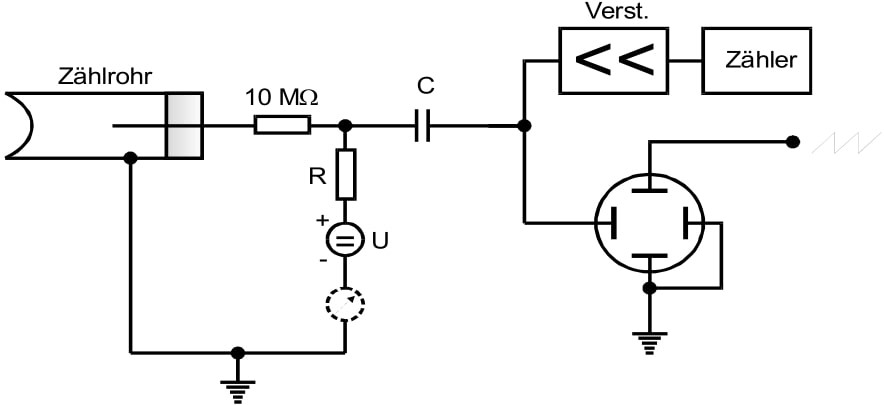
\includegraphics[width=\linewidth]{images/Aufbau.jpg}
        \caption{Aufbau des Geiger-Müller Zählrohrs samt Messaparatur \cite{V703}}
        \label{fig:5}
    \end{figure}

    \flushleft{Dabei\;}\justifying sollte die maximale Impulsrate $\SI{100}{\per\second}$ Impulse nicht überschreiten. Die Impulsrate wird
    bei einer Startspannung von $\SI{320}{\volt}$ und fortlaufend in $\SI{10}{\volt}$-Schritten gemessen. Die Integrationszeit pro 
    Zählrohrspannung beträgt $\SI{60}{\second}$. Die Messungen werden bis zu einer Zählrohrspannung von $\SI{700}{\volt}$ durchgeführt. Dabei
    ist es wichtig zu beachten, dass die $\SI{700}{\volt}$ nicht überschritten werden dürfen, da das Zählrohr sonst zerstört werden würde.
    Neben der Impulsrate wird außerdem der Strom in $\SI{50}{\volt}$-Schritten dem Amperemeter entnommen.

    \flushleft{Um\;}\justifying die Totzeit des Geiger-Müller Zählrohrs zu erhalten, werden die Zwei-Quellen- und Oszilloskopmethode verwendet. 
    Für die Zwei-Quellen-Methode wird zuerst die $^{204}$Tallium-Quelle näher an das Geiger-Müller Zählrohr bewegt. Anschließend wird das zweite 
    Präparat hinzugestellt. Abschließend wird das erste Präparat entfernt. Für jeden der drei Schritte wird eine Integrationszeit von $\SI{120}
    {\second}$ verwendet. 

    \newpage
    \flushleft{Für\;}\justifying die Oszilloskopmethode wird die Zeit zwischen den ersten beiden Pulsen von dem folgenden Bild abgelesen:

    \begin{figure}[H]
        \centering
        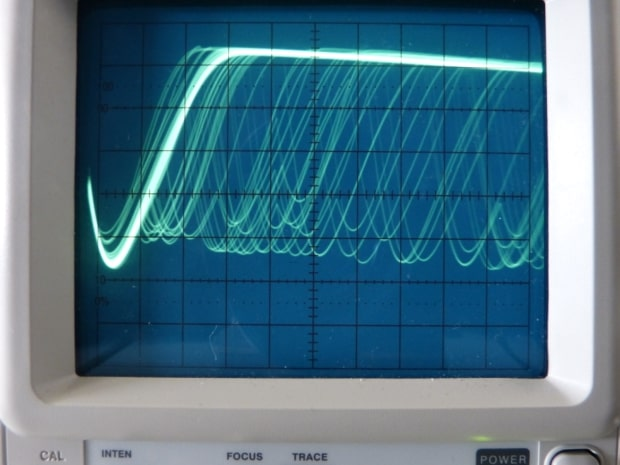
\includegraphics[width=0.75\linewidth]{images/Oszilloskop.jpg}
        \caption{Momentaufnahme des Oszilloskops \cite{V703}}
        \label{fig:6}
    \end{figure}

    \flushleft{Dabei\;}\justifying beträgt eine Kästchenlänge der Zeitachse $\SI{100}{\micro\second}$. 

\newpage
\section{Auswertung}

    \subsection{Zählrohrcharakteristik}

    \flushleft{Der\;}\justifying folgende Graph beschreibt die Zählrohrcharakteristik und beinhaltet die Plateaulänge und Steigung
    symbolisiert bei der linearen Ausgleichsrechnung. Für die Erstellung des Graphen wurden die Werte der Tabelle \ref{tab:1} und 
    die Pythonbibliothek matplotlib \cite{matplotlib}, bzw. der Pythonbefehl polyfit \cite{numpy} für die Ausgleichsgerade verwendet. 
    Hierbei ist zu beachten, dass die Werte der Impulsrate $N$ Poisson verteilt sind, wodurch sich ein Fehler $\Delta N = \sqrt{N}$ 
    ergibt, welcher an die Messwerte über Python als ufloat \cite{uncertainties} übergeben werden. Dieser Fehler wird im folgenden 
    Graphen als vertikaler Balken aufgetragen.

    \begin{figure}[H]
        \centering
        \includegraphics[width=\textwidth]{build/plotGM.pdf}
        \caption{Zählrohrcharakteristik}
        \label{fig:7}
    \end{figure}

    \flushleft{Die\;}\justifying für die Ausgleichsgerade $N = m*U+b$ relevanten Parameter der Steigung $m$ und des Schnittpunkts der y-Achse 
    $b$ lauten wie folgt:
    \begin{align}
        m &= \text{\input{m_GM.tex}}\\
        b &= \text{\input{b_GM.tex}}
    \end{align}

    \subsection{Totzeit}

    \flushleft{Für\;}\justifying die Bestimmung der Totzeit $T$ mithilfe der Zwei-Quellen-Methode werden die jeweiligen Impulsraten der
    einzelnen Quellen benötigt. Diese lauten
    wie folgt \cite{V703}:
    \begin{align}
        N_1 &= \text{\input{N_1.tex}}\\
        N_2 &= \text{\input{N_2.tex}}\\
        N_{1+2} &= \text{\input{N_12.tex}}
        \intertext{\flushleft{Mithilfe\;}\justifying dieser Impulsraten und der Formel \eqref{eq:3} lässt sich die folgende Totzeit bestimmen:
        }
        T &\approx \text{\input{T.tex}}
    \end{align}
    \flushleft{Für\;}\justifying die Oszilloskopmethode werden der Primärimpuls und der Sekundärimpuls aus Abbildung \ref{fig:6} abgelesen. Hierbei
    ist die Länge eines Kastens \SI{100}{\micro\second}. Die Zeitdifferenz bezeichnet die Totzeit und lautet:
    \begin{align}
        T &\approx \SI{50}{\micro\second}
    \end{align}
    \flushleft{Aufgrund\;}\justifying der Auflösung und der Menge der Impulsen ist es schwer den Primärimpuls und Sekundärimpuls zu bestimmen. Hier ist der
    Primärimpuls der prominente Impuls (ca. \SI{120}{\micro\second} von links) und der Sekundärimpuls der daurauf folgende Impuls (ca. \SI{170}
    {\micro\second} von links).

    \subsection{Zahl der freigesetzten Ladungen pro einfallendem Teilchen}

    \flushleft{Die\;}\justifying Zahl der freigesetzten Ladungen pro einfallendem Teilchen $Z$ lässt sich mit der Formel \eqref{eq:5} und 
    den Werten der Impulsraten aus Tabelle \ref{tab:2} bestimmen. 
    Dazu wird die jeweilige Stromstärke $I$ benötigt. Die Werte für $Z$ mit ihrer zugehörigen Stromstärke sind in der folgenden Tabelle aufgetragen:

    \begin{table}[H]
        \centering
        \input{Z.tex}
        \caption{Freigesetzte Ladungen pro einfallendem Teilchen $Z$ und dessen Strom $I$}
        \label{tab:3}
    \end{table}
    \flushleft{Beide\;}\justifying Werte sind hier fehlerbehaftet, da die Stromstärke $I$ einem Fehler von $\Delta I = \SI{0.05}{\micro\second}$
    unterliegt. Werden die Werte für $Z$ und dessen Stromstärke $I$ graphisch gegeneinander aufgetragen (wieder mit der Pythonbibliothek matplotlib
    \cite{matplotlib}), ergibt sich der folgende Graph:
    \begin{figure}[H]
        \centering
        \includegraphics[width=\textwidth]{build/plotZ.pdf}
        \caption{$Z$ als Funktion des Stroms $I$}
        \label{fig:8}
    \end{figure}
    \flushleft{Da\;}\justifying hier beide Werte fehlerbehaftet sind, hat jeder Messwert einen Fehlerbalken in x- und y-Richtung. Es wird 
    mithilfe der Geradengleichung $Z=m*I+b$ und dem Pythonbefehl polyfit \cite{numpy} eine Ausgleichsgerade durch alle Messwerte gelegt. 
    Die dazugehörigen Parameter $m$ und $b$ lauten wie folgt:
    \begin{align}
        m &= \text{\input{m.tex}}\\
        b &= \text{\input{b.tex}}
    \end{align}

\newpage
\section{Diskussion}

    \flushleft{Der\;}\justifying Graph der Zählrohrcharakteristik \ref{fig:7} gibt einen Zählratenverlauf ähnlich zu dem erwarteten Verlauf
    aus Abbildung \ref{fig:4} aus. Die Impulsrate $N$ muss hier bei ca. $\SI{10000}{\per\second}$ gehalten werden, da der Fehler bei 
    $\leq \SI{1}{\percent}$ liegen soll. Im Graphen \ref{fig:7} ist der abrupte Anstieg der Zählrate an den letzten vier Werten erkennbar. Verglichen mit der Abbildung
    \ref{fig:4} stellt die in der Zählrohrcharakteristik abgebildete Ausgleichsgerade ein gutes Plateau dar, da die ersten drei und die letzten vier
    Messwerte nicht in die Rechnung der Ausgleichsgerade miteinbezogen werden. Diese Werte beschreiben die an dem Plateau angrenzenden
    Spannungsbereiche $U_E$ und der Dauerentladung. Eine Steigung des Plateaus von $m = \text{\input{m_GM.tex}}$ entspricht gleichermaßen der 
    erwarteten Steigung, da idealerweise die Steigung gleich null sein sollte, es aber aufgrund der dennoch auftretenden Nachentladung eine 
    geringe Steigung gibt. 

    \flushleft{Die\;}\justifying Totzeit der ZQM nach Formel \eqref{eq:3} gibt einen realistischen Wert wieder. Dies wird bestätigt, wenn die Totzeit 
    mit der des Zählrohrs aus Versuch 603 von $\SI{90}{\micro\second}$ \cite{V603} verglichen wird. Wenn die Zählrate $N_{1+2}$ mit der Summer der
    Zählraten $N_1$ und $N_2$ verglichen wird, stellt sich heraus, dass die Bedingung $N_{1+2} < N_1+N_2$ hier erfüllt ist. Die OM hingegen lässt auf keinen nützlichen
    Wert schließen, da nicht klar zwischen Primär- und Sekundärimpuls unterschieden werden kann. Demnach ist die Totzeit $T=\SI{50}{\micro\second}$
    nicht realistisch. 

    \flushleft{Der\;}\justifying Graph \ref{fig:8} und dessen Ausgleichsgerade gibt eine fast lineare Beziehung der einzelnen Messwerte wieder. 
    $Z$ wächst mit einem steigenden Strom, wobei die letzten drei Werte stärker von der Ausgleichsgeraden abweichen. Der Fehler der beiden Werte
    setzt sich größtenteils aus dem Messfehler des Amperemeters und dem statistischen Fehler der Impulsrate zusammen.

\newpage
\printbibliography

\newpage
\section{Appendix}

    \input{GM.tex}

    \begin{table}[H]
        \centering
        \input{strom.tex}
        \caption{Messwerte des Zählerstroms des Geiger-Müller Zählrohrs}
        \label{tab:2}
    \end{table}

\end{document}